\documentclass[12pt,3p]{article}
\usepackage[T1]{fontenc}
\usepackage[utf8]{inputenc}
\usepackage[english]{babel}
\usepackage[margin=0.75in]{geometry}
\usepackage{amsmath}
\usepackage{mathtools}
\usepackage{enumitem}
\usepackage{physics}
\usepackage{bm}

\usepackage[round,numbers]{natbib}
\usepackage[colorlinks = false]{hyperref}

\begin{document}

\title{\Large{FEniCS: 2D Linear Elasticity} \\
	\large{Based on Numerical Tours of Continuum Mechanics Using FEniCS} \vspace{-2ex}}

\author{Ida Ang: Edited \today}
\date{\vspace{-5ex}}
\maketitle

\tableofcontents
\newpage

\section{Problem Definition}
\vspace{-2ex}
This demonstration shows how to compute a small strain solution for a 2D isotropic linear elastic medium in either plane stress or plane strain, in a traditional displacement based finite element formulation. 

This document is meant to provide additional information that supplements the  \href{https://comet-fenics.readthedocs.io/en/latest/demo/elasticity/2D_elasticity.py.html}{2D linear elasticity demonstration} on \href{https://comet-fenics.readthedocs.io}{Numerical Tours of Computational Mechanics with FEniCS} , but still assumes the reader has a basic understanding of common solid mechanics notations (ie. indicial notation). 

Several modification are made, some of which are purely for convenience and usability. For example, 1) parameters can now be parsed in from command line for running different cases (ie, plane strain vs plane stress). For convergence purposes, 2) the body force can be ramped from a low to high value within a for loop. 3) Post-processing of final values are included to demonstrate code functionality and comparison to an analytical solution

\section{Formulation}
\vspace{-2ex}

Equation for strain in terms of displacement
\begin{subequations}\label{Strain}
\begin{align}
\epsilon_{ij} &= \frac{1}{2} (\pdv{u_i}{x_j} + \pdv{u_j}{x_i}) \\
 \bm{\epsilon} &= \frac{1}{2} (\nabla \mathbf{u} + \nabla \mathbf{u}^T)
\end{align}
\end{subequations}
General expression of the linear elastic isotropic constitutive relationship 
\begin{equation}\label{EqStressStrain}
\sigma_{ij} = \lambda \epsilon_{kk} \delta_{ij} + 2 \mu \epsilon_{ij}
\end{equation}
Equation \ref{EqStressStrain} can be inverted,
\begin{equation}\label{EqStrainStress}
\epsilon_{ij} = \frac{1+ \nu}{E} \sigma_{ij} - \frac{v}{E} \sigma_{kk} \delta_{ij}
\end{equation}
where the Lamé coefficients are given by: 
\begin{align}\label{EqLame}
\begin{split}
\lambda &= \frac{E \nu}{(1+ \nu) (1 - 2 \nu)} \\
\mu &= \frac{E}{2 (1+ \nu)}
\end{split}
\end{align}
The user will be able to specify either a plane strain or stress condition in the code. See the subsections below 

\subsection{Plane Strain}
The strain tensor under plane strain assumptions: 
\begin{equation*}
\bm{\epsilon} = 
\begin{bmatrix}
\epsilon_{xx} & \epsilon_{xy} & 0 \\
\epsilon_{yx} & \epsilon_{yy} & 0 \\
0 & 0 & 0 \\
\end{bmatrix}
\end{equation*}
Eq. \ref{EqStressStrain} for plane strain gives the following relationship for $\sigma_{ij}$
\begin{align}\label{EqPlaneStrain}
\begin{split}
\sigma_{ij} &= \lambda \epsilon_{kk} \delta_{ij} + 2 \mu \epsilon_{ij} \\
\sigma_{ij} &= \lambda (\epsilon_{xx} + \epsilon_{yy} + \epsilon_{zz}) + 2 \mu \epsilon_{ij} \quad \text{where } \epsilon_{zz} = 0 
\end{split}
\end{align}
Therefore, the constitutive relationship for plane strain is given as follows, 
\begin{equation}\label{EqPlaneStrain}
\sigma_{\alpha \beta} = \lambda (\epsilon_{xx} + \epsilon_{yy}) + 2 \mu \epsilon_{\alpha \beta} 
\end{equation}
where the change to the indices indicates $\alpha, \beta \in 1, 2$ and $i, j \in 1, 2, 3$

\subsection{Plane Stress}
The stress tensor under plane stress assumptions
\begin{equation*}
\sigma = 
\begin{bmatrix}
\sigma_{xx} & \sigma_{xy} & 0 \\
\sigma_{yx} & \sigma_{yy} & 0 \\
0 & 0 & 0 \\
\end{bmatrix}
\end{equation*}
Eq. \ref{EqStressStrain} for plane stress gives the following relationship for $\epsilon_{zz}$
\begin{align*}
\sigma_{ij} &= \lambda \epsilon_{kk} \delta_{ij} + 2 \mu \epsilon_{ij} \\
0 &= \lambda (\epsilon_{xx} + \epsilon_{yy} + \epsilon_{zz}) + 2 \mu \epsilon_{zz} \\
- (2 \mu + \lambda) \epsilon_{zz} &= \lambda (\epsilon_{xx} + \epsilon_{yy}) \\
\epsilon_{zz} &= -\frac{\lambda}{(2 \mu + \lambda)} (\epsilon_{xx} + \epsilon_{yy})
\end{align*}
Write a general form of the constitutive relationship by substituting the above into Eq. \ref{EqStressStrain}: 
\begin{align*}
\sigma_{ij} &= \lambda \epsilon_{kk} \delta_{ij} + 2 \mu \epsilon_{ij} \quad \text{where } \epsilon_{kk} = \epsilon_{xx} + \epsilon_{yy} + \epsilon_{zz} \\
\sigma_{ij} &= \lambda \bigg[ \epsilon_{xx} + \epsilon_{yy} - \frac{\lambda}{2 \mu + \lambda} (\epsilon_{xx} + \epsilon_{yy}) \bigg]  + 2 \mu \epsilon \\
&= \lambda \big[ 1 - \frac{\lambda}{\lambda + 2 \mu } \big] (\epsilon_{xx} + \epsilon_{yy} ) + 2 \mu \epsilon 
\end{align*}
Therefore, the constitutive relationship for plane stress is given as follows, 
\begin{equation}\label{EqPlaneStress}
\sigma_{\alpha \beta} = \frac{2 \lambda \mu}{\lambda + 2 \mu } (\epsilon_{xx} + \epsilon_{yy} ) + 2 \mu \epsilon 
\end{equation}
where the change to the indices indicates $\alpha, \beta \in 1, 2$ and $i, j \in 1, 2, 3$

\subsection{Strong to Weak Form}
Starting from the mechanical equilibrium equation, or strong form,
\begin{subequations}\label{EqStrongForm}
\begin{align}
- \text{Div} \bm{\sigma} = \mathbf{f} \quad \rightarrow - \div \bm{\sigma} &= \mathbf{f} \\
	\bm{\sigma} \cdot \textbf{n} &= \mathbf{t} 
\end{align}
\end{subequations}
where $\bm{\sigma}$ is the Cauchy stress, $\mathbf{f}$ is the body force, and $\mathbf{t}$ is the traction force. Eq. \ref{EqStrongForm}b for traction is also known as the Neumann or natural boundary condition which is naturally subsumed into the weak form in the following derivation. First, Eq. \ref{EqStrongForm} is converted to indicial notation,
\begin{align*}
\begin{split}
- \pdv{}{x_k} \mathbf{e_k} \cdot \sigma_{ij} (\mathbf{e_i} \otimes \mathbf{e_j}) &= f_k \mathbf{e_k} \\
- \pdv{\sigma_{ij}}{x_k} \delta_{ki} \mathbf{e_j} &= f_k \mathbf{e_k} \\
- \pdv{\sigma_{ij}}{x_i} \mathbf{e_j} &= f_k \mathbf{e_k} \quad \text{Multiply be a test function} \\
- \pdv{\sigma_{ij}}{x_i} \mathbf{e_j} \cdot v_p \mathbf{e_p} &= f_k \mathbf{e_k} \cdot v_p \mathbf{e_p} \\
- \pdv{\sigma_{ij}}{x_i} v_p \delta_{jp} &= f_k v_p \delta_{kp} \\
		 - \pdv{\sigma_{ij}}{x_i} v_j &= f_k v_k \quad \text{Integrate over domain} \\
 - \int_{\Omega} \pdv{\sigma_{ij}}{x_i} v_j dx &= \int_{\Omega} f_k v_k dx \\
\end{split}
\end{align*}
Integration by parts on the left hand side
\begin{align*}
(fg)' = f'g + fg' \rightarrow f'g &= (fg)' - fg' \\
\pdv{\sigma_{ij}}{x_i} v_j &= (\sigma_{ij} v_j)_{,i} - \sigma_{ij} \pdv{v_j}{x_i} 
\end{align*}
Substitute the result from integration by parts: 
\begin{align*}
\begin{split}
- \int_{\Omega} (\sigma_{ij} v_j)_{,i} dx + \int_{\Omega} \sigma_{ij} \pdv{v_j}{x_i} dx &= \int_{\Omega} f_k v_k dx \quad \text{Use the divergence theorem} \\ 
- \int_{\partial \Omega} \sigma_{ij} v_j n_i ds + \int_{\Omega} \sigma_{ij} \pdv{v_j}{x_i} dx &= \int_{\Omega} f_k v_k dx \quad \text{Recognize the traction term} \\
- \int_{\partial \Omega} t_i v_j ds + \int_{\Omega} \sigma_{ij} \pdv{v_j}{x_i} dx &= \int_{\Omega} f_k v_k dx \quad \text{Rearrange} \\
 \int_{\Omega} \sigma_{ij} \pdv{v_j}{x_i} dx &= \int_{\Omega} f_k v_k dx + \int_{\partial \Omega} t_i v_j ds
\end{split}
\end{align*}
The principle of virtual work states that:
\begin{equation}\label{PVW}
\int_{\Omega} \delta W dV = \int_{\Omega} \sigma_{ij} \delta \epsilon_{ij} dV = \int_{\partial \Omega} t_i \delta u_i dS + \int_{\Omega} b_i \delta u_i dV 
\end{equation}
Applying this principle to, where $\mathbf{f}$ is  the body force: 
\begin{align*}
 \int_{\Omega} \sigma_{ij} \pdv{v_j}{x_i} dx &= \int_{\Omega} f_k v_k dx + \int_{\partial \Omega} t_i v_j ds \\
 \int_{\Omega} \sigma_{ij} \epsilon_{ij} dV &= \int_{\Omega} f_k v_k dx + \int_{\partial \Omega} t_i v_j ds \quad \text{no traction applied} \\
  \int_{\Omega} \sigma_{ij} \epsilon_{ij} dV &= \int_{\Omega} f_k v_k dx
\end{align*}
Writing in direct notation, we have the variational (weak) formulation. Find $\mathbf{u} \in V$ such that: 
\begin{equation}\label{EqWeakForm}
\int_{\Omega}  \bm{\sigma}(\mathbf{u}) : \bm{\epsilon}(\mathbf{v}) \, d \Omega = \int_{\Omega} \mathbf{ f \cdot v } \, d \Omega \quad \forall \mathbf{v} \in V 
\end{equation}

\section{FEniCS Implementation}
\vspace{-2ex}
User parameters were added to allow for specification from the command-line prompt \\
{\fontfamily{qcr}\selectfont
parameters.parse() \\
userpar = Parameters("user") \\
userpar.add("model", "plane\_stress") \\
userpar.parse() \\ \\
}
Next, user parameters can be specified by typing in the command line prompt \\
{\fontfamily{qcr}\selectfont
python3 Demo2DLE.py - -model plane\_stress \\
}
(no space between dashes), where any number of user parameters can be added and specified. \\
{\fontfamily{qcr}\selectfont
python3 Demo2DLE.py - -model plane\_stress - -MaxStep 20 - -MaxRho 0.2
}

\subsection{Validation with Analytical Solution}
We can validate our problem according to the analytical solution from Euler-Bernoulli beam theory 
\begin{equation}\label{beam}
w_{beam} = \frac{q L^4}{8 EI}
\end{equation}
where $w_{beam}$ is the overall deflection of the beam, q is a distributed load, E is Young's modulus, and I is the inertia defined as 
\begin{equation*}
I = \frac{1}{12} L H^3
\end{equation*}
We want to define the distributed load, q, in terms of our knowns. Note that the force, $f$, is defined where f and L are perpendicular
\begin{equation*}
q = f \cross L \rightarrow q = fL
\end{equation*}
Using the inertia and definition for q in Eq. \ref{beam}
\begin{align*}
w_{beam} &= \frac{q L^4}{8 E} \frac{12}{LH^3} \\
		&= \frac{3 q L^3}{E H^3} \quad \text{Substitute in } q=fL\\
w_{beam} &= \frac{3 f L^4}{E H^3}
\end{align*}
The percentage error is quantified using the following equation, where S denotes simulation deflection and A denotes the analytical solution. 
\begin{align*}
\% \, \text{Error} = 100 \, \frac{ abs |w_{S} - w_{A}| }{w_{S}}
\end{align*}
Fig. \ref{FigPlaneStrainStress} demonstrates the difference between the simulation result and analytical prediction for an increasing body force. Euler-Bernoulli beam theory has several assumptions, some of which include the assumption of linear elasticity and plane sections remaining plane. As more body force is applied, a larger displacement results in strains larger than the assumptions of linear elasticity (~5 \% strain).
\begin{figure*}[!htb]
\centering
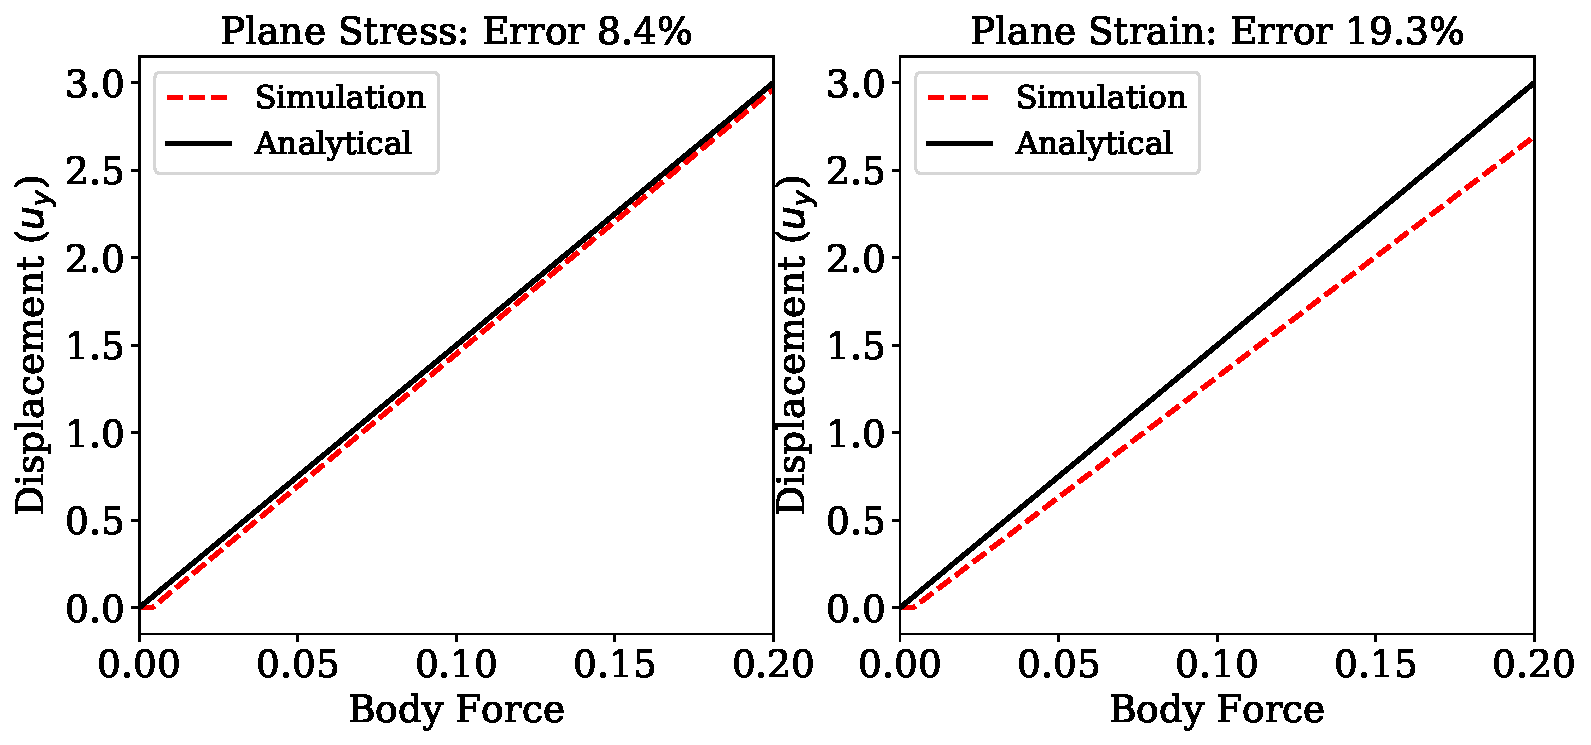
\includegraphics[width=0.8\textwidth]{./Images/PlaneStrainVsStress.pdf}
\caption{Difference between the simulation and analytical solution for a) Plane Stress and b) Plane Strain for a bar where $E = 1000, \, \nu = 0.3$. Average percentage error for every time step is quantified in the title.  }
\label{FigPlaneStrainStress}
\end{figure*}


\end{document}
